\documentclass[10pt,letter]{article}
\usepackage{amssymb,graphicx,amsmath,mathtools,ifthen,textcomp,enumerate,units,cancel}
\usepackage[margin=1.5in]{geometry}
\usepackage[T1]{fontenc}
\usepackage{tikz}
\numberwithin{equation}{section}
\newcommand{\problemdivider}{\begin{center}\large \bf\ldots\ldots\ldots\ldots\ldots\ldots\end{center}}
\newcommand{\subproblemdivider}{\begin{center}\large \bf\ldots\ldots\end{center}}
\newcommand{\pdiv}{\problemdivider}
\newcommand{\spdiv}{\subproblemdivider}
\newcommand{\ba}{\begin{align*}}
\newcommand{\ea}{\end{align*}}
\newcommand{\rt}{\right}
\newcommand{\lt}{\left}
\newcommand{\bp}{\begin{problem}}
\newcommand{\ep}{\end{problem}}
\newcommand{\bsp}{\begin{subproblem}}
\newcommand{\esp}{\end{subproblem}}
\newcommand{\bssp}{\begin{subsubproblem}}
\newcommand{\essp}{\end{subsubproblem}}
\newcommand{\atag}[1]{\addtocounter{equation}{1}\label{#1}\tag{\arabic{section}.\alph{subsection}.\alph{equation}}}
\newcommand{\btag}[1]{\addtocounter{equation}{1}\label{#1}\tag{\arabic{section}.\alph{equation}}}
\newcommand{\ctag}[1]{\addtocounter{equation}{1}\label{#1}\tag{\arabic{equation}}}
\newcommand{\unts}[1]{\ \text{#1}}
\newcommand{\textop}[1]{\operatorname{#1}}
\newcommand{\textopl}[1]{\operatornamewithlimits{#1}}
\newcommand{\prt}{\partial}
\newcommand{\pderi}[3]{\frac{\prt^{#3}#1}{\prt #2^{#3}}}
\newcommand{\deri}[3]{\frac{d^{#3}#1}{d #2^{#3}}}
\newcommand{\del}{\vec\nabla}
\newcommand{\exval}[1]{\langle #1\rangle}
\newcommand{\bra}[1]{\langle #1|}
\newcommand{\ket}[1]{|#1\rangle}
\newcommand{\ham}{\mathcal{H}}
\newcommand{\arr}{\mathfrak{r}}

\newcommand{\bsm}{\lt(\begin{smallmatrix}}
\newcommand{\esm}{\end{smallmatrix}\rt)}
\newcommand{\bpm}{\begin{pmatrix}}
\newcommand{\epm}{\end{pmatrix}}
\newcommand{\bdet}{\lt|\begin{smallmatrix}}
\newcommand{\edet}{\end{smallmatrix}\rt|}

\newcommand{\bs}[1]{\boldsymbol{#1}}
\newcommand{\uvec}[1]{\bs{\hat{#1}}}

\newcommand{\qed}{\hfill$\Box$}

\def\thesection{\textbf{\arabic{section}}}
\def\thesubsection{\textbf{\thesection.\alph{subsection}.}}
\def\thesubsubsection{\textbf{\alph{subsubsection}.}}

\makeatletter
\newenvironment{problem}[1]{\ifthenelse{\arabic{section}>0}{\pdiv}{}\@startsection
       {section}
       {1}
       {0em}
       {0em}
       {0em}
       {\pagebreak[3]}{\bf #1}\hspace{3mm}}
       {}
\newenvironment{subproblem}[1]{\ifthenelse{\arabic{subsection}>0}{\spdiv}{}\@startsection
       {subsection}
       {2}
       {0em}
       {0em}
       {0em}
       {\pagebreak[3]}{\it #1}.}
       {}
\newenvironment{subsubproblem}{\@startsection
       {subsubsection}
       {3}
       {0em}
       {0em}
       {0em}
       {\pagebreak[3]}}
       {}
\makeatother


\begin{document}
\noindent\textbf{\textsc{HapASeg}}\\
\noindent\textsc{Julian Hess}\\
\noindent 16 August 2021\\

\section{Motivation}

In order to perform cancer phylogenetic analyses, we need extremely accurate CNV calls, since phylogenetic analyses depend on accurate estimation of mutations' CCFs, which in turn depends on accurate estimation of the absolute/subclonal allelic copy numbers at the loci of each mutation. Calling absolute allelic copy number requires accurate calls for both total copy ratio (i.e., the relative amount of genomic mass at each genomic locus) and allelic imbalance (i.e., the relative abundance of one allele versus the other allele at each locus).

Unfortunately, CNV callers have not kept pace with the demands of the field. I see two fundamental flaws with current CNV calling approaches. The first is that they use total copy ratio segmentation, as inferred from genomic coverage, as the primary signal. Genomic coverage carries many systematic biases, which cannot be easily corrected \textit{a priori}. A typical solution is to use a large panel of normals (PoN) to empirically correct for these biases---because these are assumed to be diploid almost everywhere, any systematic fluctuations in their coverage are due to technical artifacts. However, therein lies the second fundamental flaw: the panel of normals must be matched exactly to the sequencing technology and protocol being used to assay the tumor, since each protocol will have its own biases. Assembling PoNs can be tricky, since tumor samples are often of types not typical to normal samples (e.g., FFPE, cfDNA), and properly matching samples to a good PoN adds additional complexity to analyses.

I propose to address this issue by using allelic imbalance segmentation as the primary signal. Allelic imbalance is much less prone to systematic biases, and by incorporating prior phasing information, is extremely robust even at low purities. We will first discuss methods for probabilistically segmenting allelic imbalance, clustering non-adjacent segments into discrete sample-wide levels of imbalance, and finally, leveraging these clusters as a strong prior for total copy ratio segmentation.

\section{Allelic segmentation intro}

\begin{figure}
\centering
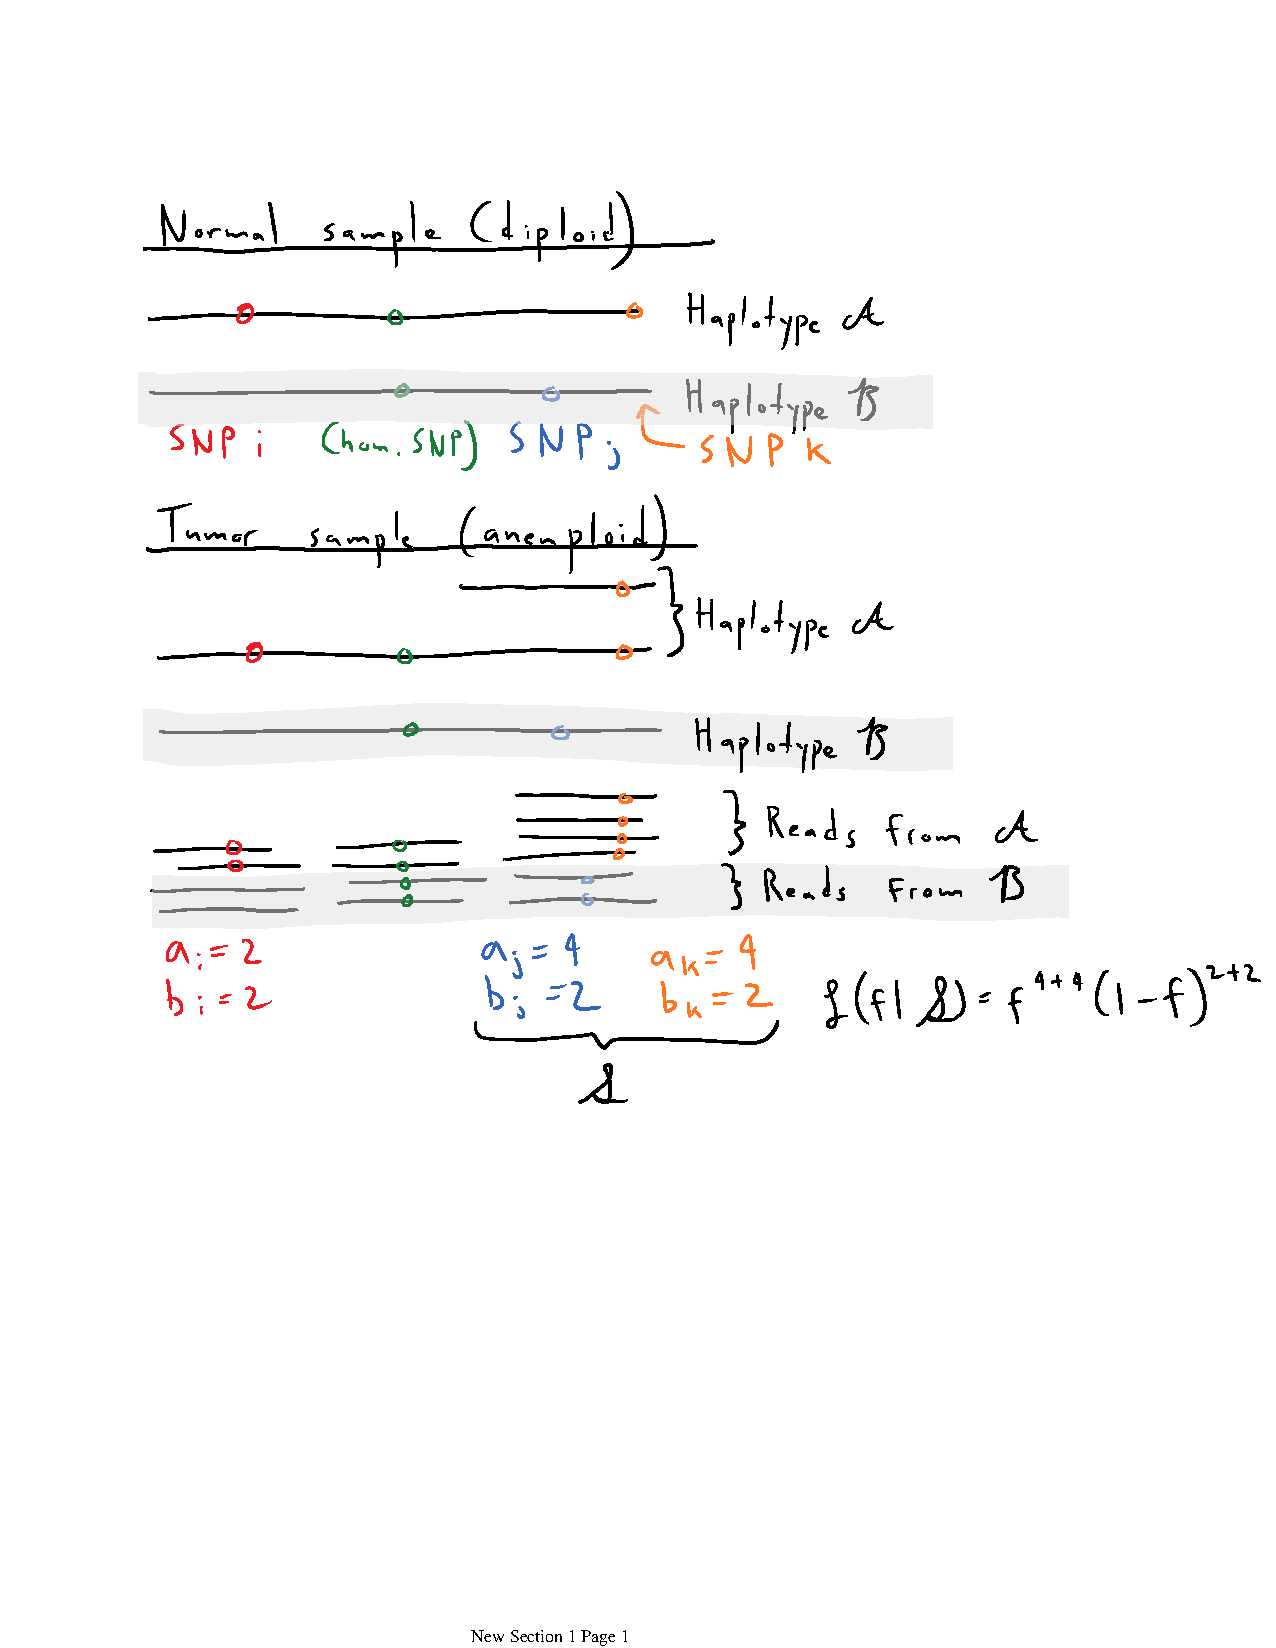
\includegraphics[trim={2cm 9cm 0 3cm},clip,width=10cm]{Figs/fig1.pdf}
\caption{A depiction of how phased SNPs' readcounts get translated to phased allele counts $a$ and $b$.}
\label{introfig}
\end{figure}

Consider a set $\mathcal{S}$ of phased SNPs on haplotypes $\mathcal{A}$ and $\mathcal{B}$. SNP $i$ assigned to $\mathcal{A}$ has alternate read count $a_i$ and reference read count $b_i$, while SNP $j$ assigned to $\mathcal{B}$ has alternate read count $b_j$ and reference read count $a_j$. We can express the allelic imbalance $f$ of $\mathcal{S}$ in terms of the relative fraction of $\mathcal{A}$, which we call the ``haplotypic imbalance.'' In a diploid region of the genome, $f = 1/2$. In a triploid region with two copies of $\mathcal{A}$ and one copy of $\mathcal{B}$, $f = 2/3$, given 100\% tumor purity, (Figure \ref{introfig}).

Assuming only aleatoric uncertainty, the likelihood of the haplotypic imbalance $f$ for all SNPs in $\mathcal{S}$ is
\begin{align*}
\mathcal{L}(f|\mathcal{S}) &= \prod_{i\in\mathcal{S}} f^{a_i} (1 - f)^{b_i}\\
&= f^{\sum_{i\in\mathcal{S}} a_i}(1-f)^{\sum_{i\in\mathcal{S}} b_i}\\
&\equiv f^{A_\mathcal{S}}(1-f)^{B_\mathcal{S}}\btag{As}
%&\propto \textop{beta}\lt(1 + \textstyle\sum_{i\in\mathcal{S}} a_i, 1 + \sum_{i\in\mathcal{S}}  b_i\rt)\\
%&\equiv f\sim\textop{beta}(1 + A_\mathcal{S}, 1 + B_\mathcal{S})
\end{align*}
where $A_\mathcal{S}$ and $B_\mathcal{S}$ are the total read counts respectively assigned to $\mathcal{A}$ and $\mathcal{B}$ within segment $\mathcal{S}$. Since the SNPs are ordered along a chromosome, we can parameterize $\mathcal{S}$ in terms of the disjoint intervals defining each segment. Denote the genomic position of SNP $i$ as $x_i$, and the set of all SNPs as $\mathcal{X}$. For a given half-open genomic interval $[s_j,e_j)$, with $s_{j+1}=e_j$ and $s_1=1$, we have
\begin{align*}
\mathcal{L}(f_j,[s_j,e_j)|\mathcal{X})=\prod_{\mathclap{\{i|x_i\in [s_j, e_j)\}}} f_j^{a_i}(1 - f_j)^{b_i}
\end{align*}
which is equivalent to \eqref{As} above. Marginalizing out $f_j$ yields
\begin{align*}
\mathcal{L}([s_j,e_j)|\mathcal{X})&=\int_0^1 df_j\,\prod_{\mathclap{\{i|x_i\in [s_j, e_j)\}}} f_j^{a_i}(1 - f_j)^{b_i}\\
&= \beta(A_{\mathcal{S}_j}+1, B_{\mathcal{S}_j}+1)
\end{align*}
where $\beta$ is the beta function.

Our goal is to find a good allelic segmentation. This requires finding the optimal partition of all SNPs, i.e.\ the optimal set of $\{[s,e)\}$ that maximizes the marginal likelihood
\begin{align*}
\mathcal{L}(\{[s,e)\}|\mathcal{X})=\prod_j \mathcal{L}([s_j,e_j)|\mathcal{X}).
\end{align*}
Unfortunately, for $N$ total SNPs, the total number of possible partitions is $2^N$. Luckily, the space of partitions is amenable to sampling via MCMC. While this won't give us the exact optimal partition, it gives us something even better: the posterior probability of segmentations.

\section{Allelic segmentation MCMC}
\label{MCMC_section}

Initially, each SNP belongs to its own segment. At random, we pick two adjacent segments and probabilistically merge them according to the Metropolis criterion:
\begin{align*}
\textop{Pr}(\underbrace{[s_j,e_j),[s_{j+1},e_{j+1})}_{S}\to \underbrace{[s_j,e_{j+1})}_{S^\ast}) = \min\lt\{1,\frac{\mathcal{M}(S^\ast)q(S|S^\ast)}{\mathcal{M}(S)q(S^\ast|S)}\rt\},\btag{metro}
\end{align*}
where marginal likelihoods are
\begin{align*}
\mathcal{M}(S^\ast) &= \beta(\underbrace{\textstyle\sum_{\{i|x_i\in [s_j, e_{j+1})\}}a_i}_{A_{[s_j,e_{j+1})}}+1,\underbrace{\textstyle\sum_{\{i|x_i\in [s_j, e_{j+1})\}}b_i}_{B_{[s_j,e_{j+1})}}+1)\btag{psum_1}\\
\mathcal{M}(S) &= \beta(A_{[s_j,e_j)}+1,B_{[s_j,e_j)}+1)\times \beta(A_{[s_{j+1},e_{j+1})}+1,B_{[s_{j+1},e_{j+1})}+1).\btag{psum_2}
\end{align*}
We can also split segments of length $>1$. Rather than picking a breakpoint within the segment at random, we probabilistically tailor our proposal distribution. For each position $k\in [s_j,e_j)$, we compute
\begin{align*}
\mathcal{L}_j(k) = \beta(A_{[s_j,k)}+1,B_{[s_j,k)}+1)\times\beta(A_{[k,e_j)}+1,B_{[k,e_j)}+1),\btag{psum_3}
\end{align*}
and propose picking $k$ as the breakpoint with probability $p_j(k)=\mathcal{L}_j(k)/\sum_k \mathcal{L}_j(k)$. Our proposal distributions are
\begin{align*}
q(S|S^\ast) = \frac{p_j(k)}{N} \qquad q(S^\ast|S) = \frac{1}{N-1}
\end{align*}
where $N$ is the total number of segments at the current MCMC iteration.

The overall MCMC procedure is:
\begin{enumerate}
\item Initialize each SNP to belong to its own segment.
\item With equal probability, pick whether to attempt a merge or split this iteration.
\item If we choose to merge, uniformly pick segment $j$ at random from 1 to $N-1$. Probabilistically merge it with segment $j+1$ with probability defined in \eqref{metro}.
\item If we choose to split, uniformly pick $j$ at random from 1 to $N$, propose a breakpoint within $j$ via \eqref{psum_3}, and accept the proposal with probability defined as the reciprocal of \eqref{metro}. Proposing a breakpoint at the end of the segment is equivalent to not accepting any proposal at all and leaving the chain as-is.
\item A given state of the chain constitutes a sample $\psi_i$ from the overall distribution of segmentations, $\Psi$. We iterate the chain until it is burned-in, then iterate some more until a sufficient number of samples $\psi_1,\dots,\psi_n\sim\Psi$ have been collected. Because the chain moves slowly between iterations (each iteration only modifies a single segment), we ``thin'' the chain and only save every $n$th sample ($n\sim 100$). In the future, we might want to adjust the thinning amount to reflect the number of segments $N_s$ at a given point in the chain, since we expect every single segment will be modified on average once every $N_s$ iterations.
\end{enumerate}

The MCMC is extremely fast, since each iteration only involves computing partial sums in \eqref{psum_1}, \eqref{psum_2}, and \eqref{psum_3} which can be memoized between iterations. In theory, storing all possible partial sums would require $O(N^2)$ space, but in practice we only ever need blocks close to the diagonal, so the partial sum matrix can be stored sparse, with space complexity $O(\bar{N}_s\bar{B}^2)\ll O(N^2)$, where $\bar{N}_s$ is the average number of segments and $\bar{B}$ the average length of each segment. The MCMC is also efficiently parallelized: the most compute-intensive phase is at the beginning when each SNP belongs to its own segment. Blocks of adjacent SNPs are burned-in in parallel, which are then concatenated post burnin to sample the final segmentation posterior. During this step, each chromosome arm can be run in parallel, since we do not expect reliable phasing across the centromere.

\subsection{SNP pruning}

We optionally propose a third operation during each iteration: SNP pruning. Within a given segment, some SNPs' haplotypic imbalance $a_i/(a_i+b_i)$ can differ considerably from the true haplotypic imbalance of the segment, whether due to random chance or systematic bias (e.g., mapping issues, poor base qualities, etc.)

We can prune these SNPs from a segment, using an MCMC step similar to splitting a segment. For the $k$th SNP in the $j$th segment $S_j$, we compute the marginal likelihood of the segment minus SNP $k$:
\begin{align*}
\mathcal{M}^{-}_j(k) = \beta(\underbrace{A_{[s_j,e_j)} - a_k}_{A^{-k}_{[s_j,e_j)}} + 1, \underbrace{B_{[s_j,e_j)} - b_k}_{B^{-k}_{[s_j,e_j)}} + 1)\times\beta(a_k + 1, b_k + 1).
\end{align*}
Note that this is extremely similar to the likelihood of splitting a segment given in \eqref{psum_3}, with the ``segment'' being split out the single SNP $k$, which can be anywhere within $j$.

If $k$ had already been removed from $j$, the marginal likelihood of adding it back is
\begin{align*}
\mathcal{M}^{+}_j(k) = \beta(A^{-k}_{[s_j,e_j)} + a_k + 1, B^{-k}_{[s_j,e_j)} + b_k + 1).
\end{align*}

The posterior ratio for removing $k$ is
\begin{align*}
p(S_j/(S_j-k))=\frac{\mathcal{M}^{-}_j(k)}{\mathcal{M}^{+}_j(k)}\times\frac{(1 - p^{+}(k))}{p^{+}(k)},\btag{prune_postr}
%p(S_j\toS_j-k)=\min\lt\{1,\frac{\mathcal{M}^{-}_j(k)}{\mathcal{M}^{+}_j(k)}\times\frac{(1 - p^{+}(k))}{p^{+}(k)}\times\frac{q(+|-)}{q(-|+)}\rt\},\btag{prune_metro}
\end{align*}
where $p^{+}(k)$ is a prior probability of including $k$. %, and $q$ is the probability of proposing to remove/add $k$, which we will define in a bit.
The ratio for adding $k$ if it had already been removed is just the reciprocal of \eqref{prune_postr}.

To propose a SNP to prune within a segment, we enumerate the probabilities $P_R$ of removing each SNP, along with the probabilities $P_A$ of adding back any SNPs that had been previously removed:
\begin{align*}
P_R &= \{p(S_j/(S_j - k))\mid k\in S_j, k\notin R\}\\
P_A &= \{p((S_j - k)/S_j)\mid k\in S_j, k\in R\}
\end{align*}
where $R$ is the set of SNPs that had been previously removed. Let $P_{\cup}=P_R\cup P_A$. We define our proposal distribution $q$ by normalizing each member of $P_\cup$, i.e.
\begin{align*}
q(S_j-k|S_j) &= \frac{p(S_j/(S_j-k))}{\sum_{p\in P_\cup} p}\qquad k\notin R\\
q(S_j|S_j-k) &= \frac{p((S_j-k)/S_j)}{\sum_{p\in P_\cup} p}\qquad k\in R.
\end{align*}

We accept or reject a proposed removal or addition with the Metropolis criterion, defined by the product of the posterior and proposal distribution ratios. Our prior distribution can come from a panel of normals (e.g., the fraction of heterozygous normals in which the het genotype confidence is high) or the matched normal itself (e.g., the confidence that the SNP is heterozygous in the matched normal).

%\begin{align*}
%p(S_j-k\toS_j)=\min\lt\{1,\frac{\mathcal{M}^{+}_j(k)}{\mathcal{M}_j}\times\frac{(1 - p^{+}(k))}{p^{+}(k)}\times\frac{q(+|-)}{q(-|+)}\rt\}
%\end{align*}

\section{Phasing}

We impute phasing using a phased reference panel (e.g.\ 1000 Genomes). If the tool used for imputation reports per-SNP phasing probabilities (i.e., the probability that SNP $i$ is incorrectly phased with respect to $i+1$), we annotate each SNP with misphase probability $m_i$. If no per-SNP probabilities are given, we use a uniform probability $m_0$ for all SNPs. We could potentially use a fixed non-uniform prior based on genetic linkage distances.

We optionally supplement imputed phasing with read-backed phasing (RBP) obtained from the alignment. Since phase orientation is relative (e.g., the phase assignment set $\Phi=\{\phi_1=A,\phi_2=B,\phi_3=B\}$ is equivalent to its complement $\Phi_\sim=\{\phi_1=B,\phi_2=A,\phi_3=A\}$), we combine the two by taking the RBP orientation with minimum Hamming distance $d_H$ from the imputed orientation, and superseding the imputed orientation with the RBP orientation. For example, for imputed orientation phase set $I$ and RBP orientation $R$
\begin{align*}
I &= {A,A,B,B,\textcolor{red}{A},A}\\
R &= {B,B,A,A,\textcolor{red}{A},B}
\end{align*}
we would flip $R$ to $R_{\sim}$, since $d_H(I,R)=5$ but $d_H(I,R_\sim)=1$. Since $I$ and $R_\sim$ differ at one position (shown in red), the orientation at the position in $R_\sim$ would supersede the orientation in $I$, so the final phase set would be $I^\ast=A,A,B,B,B,A$. Misphase probabilities for all RBP SNPs are then set to the SNP-specific probability emitted by the phasing tool (typically $\sim 0)$. At current read lengths ($151\unit{bp}$) and fragment sizes ($\approx 400\unit{bp}$), approximately x\% of SNPs can be phased via RBP in $150\times$ exomes and y\% of SNPs in $60\times$ genomes.

\subsection{Empirical phasing correction}

Imputed phasing cannot return perfect telomere-to-telomere phase sets, due to imputation switch errors and meiotic recombination events on the parental haplotypes. We empirically correct for all switches based on the observed haplotypic imbalance segmentation: if two adjacent segments have imbalance $f$ and $1-f$, respectively, they we assume they are misphased relative to each other. While it is theoretically possible for two adjacent CNVs to have the same total copy number but different haplotypic imbalances (e.g., the first CNV has 2 copies of $A$ and 1 copy of $B$ and an immediately adjacent CNV has 1 copy of $A$ and 2 copies of $B$), we expect such events to be exceedingly rare.

For two adjacent segments $\mathcal{S}_1$ and $\mathcal{S}_2$, let $A_1$, $B_1$, $A_2$, and $B_2$ be the total readcounts assigned to haplotypes $\mathcal A$ and $\mathcal B$ in segments 1 and 2, respectively. The likelihood that two adjacent segments are correctly phased (i.e., $f$ is same for both segments) is $\mathcal{L}_{\neg\text{switch}}(f|A,B)=f^{A_1+A_2}(1-f)^{B_1+B_2}$, while the likelihood of a phase switch is $\mathcal{L}_{\text{switch}}(f|A,B)=f^{A_1 + B_2}(1-f)^{B_1+A_2}$. Since we are interested in the overall likelihood of a switch (not just for a specific value of $f$), we marginalize it out, so
\begin{align*}
\mathcal{L}_{\neg\text{switch}}(A,B)&=\int_0^1 df\,f^{A_1+A_2}(1-f)^{B_1+B_2}\\
&=\beta(A_1+A_2+1,B_1+B_2+1)\\
\mathcal{L}_{\text{switch}}(A,B)&=\int_0^1 df\, f^{A_1 + B_2}(1-f)^{B_1+A_2}\\
&=\beta(A_1+B_2+1,B_1+A_2+1).
\end{align*}

The posterior probability that the segments are misphased is obtained from Bayes's rule,
\begin{align*}
p(\text{switch}|A,B) = \frac{\mathcal{L}_{\text{switch}}(A,B)p(\text{switch})}{\mathcal{L}_{\text{switch}}(A,B)p(\text{switch})+\mathcal{L}_{\neg\text{switch}}(A,B)(1-p(\text{switch}))}.\btag{pswitch}
\end{align*}
The prior probability $p(\text{switch})$ is taken directly from the misphasing probability $m_i$ at the SNP directly upstream of the breakpoint, as reported by the imputation or RBP tool.

We wish to correct phasing because it gives us greater segmentation confidence: two adjacent segments misphased relative to each other will have higher segmental uncertainty than a single contiguous segment with the same relative phase. We must ensure that any phase corrections are performed in the same absolute direction
%(e.g., we always flip $\mathcal{B}\to\mathcal{A}$, never the other way around)
so that all corrections will result in consistent phase orientations. By convention, we will orient segments towards the ``upper'' orientation, i.e., haplotypic imbalance $f>0.5$.

For a given post-burnin MCMC iteration, we take the set of segments $\{[s_i,e_i)\}_{i=1}^{n-1}$ and for each segment compute the misphase probability
\begin{align*}
p_\text{switch}(i,i+1)=p(\text{switch}|A_{[s_i,e_i)},B_{[s_i,e_i)},A_{[s_{i+1},e_{i+1})},B_{[s_{i+1},e_{i+1})})
\end{align*}
as defined in \eqref{pswitch}. We then assign segments to absolute phase orientations upper $\mathcal{U}_i\equiv f_i > 0.5$ and lower $\mathcal{L}_i\equiv f_i < 0.5$ via the hidden Markov model shown in Figure \ref{HMMfig}, whose hidden states are the absolute phase orientations $\mathcal{U}_i$ and $\mathcal{L}_i$ and whose emissions are phased readcounts. Blue transition probabilities are $p_\text{switch}(i,i+1)$; red transition probabilities are $1 - p_\text{switch}(i,i+1)$. Black emission probabilities are the probability that the segment's mean lies above 0.5, while orange emissions are the probability that the segment's mean is less than 0.5. Because all probabilities are known, we can find the optimal HMM path via the Viterbi algorithm.

\begin{figure}
\centering
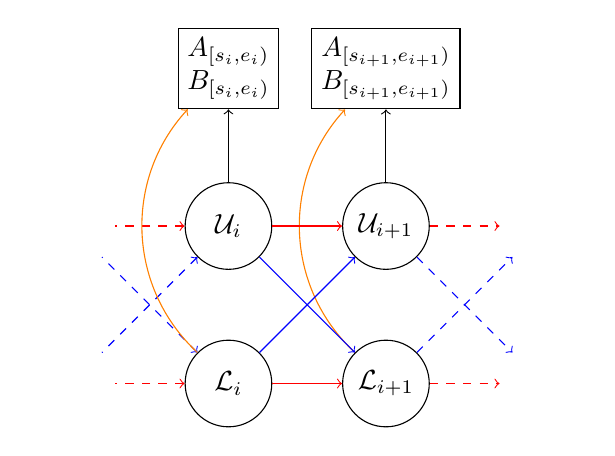
\begin{tikzpicture}
\tikzstyle{circ}=[circle,draw=black,minimum size=11mm]
\tikzstyle{circ_inv}=[circle,minimum size=11mm]
\tikzstyle{square}=[rectangle,draw=black,minimum size=10mm,align=center]
\node [circ_inv] (A0) at (-2,2) {};
\node [circ_inv] (B0) at (-2,0) {};
\node [circ_inv] (A3) at (4,2) {};
\node [circ_inv] (B3) at (4,0) {};
\node [square] (R1) at (0,4) {$A_{[s_i,e_i)}$\\$B_{[s_i,e_i)}$};
\node [square] (R2) at (2,4) {$A_{[s_{i+1},e_{i+1})}$\\$B_{[s_{i+1},e_{i+1})}$};
\node [circ] (A1) at (0,2) {$\mathcal{U}_i$}
edge [<-,dashed,red] (A0)
edge [<-,dashed,blue] (B0)
edge [->] (R1);
\node [circ] (B1) at (0,0) {$\mathcal{L}_i$}
edge [<-,dashed,red] (B0)
edge [<-,dashed,blue] (A0)
edge [->,bend left=45,color=orange] (R1);
\node [circ] (B2) at (2,0) {$\mathcal{L}_{i+1}$}
edge [<-,red] (B1)
edge [->,bend left=45,color=orange] (R2)
edge [->,dashed,red] (B3)
edge [->,dashed,blue] (A3)
edge [<-,blue] (A1);
\node [circ] (A2) at (2,2) {$\mathcal{U}_{i+1}$}
edge [<-,red] (A1)
edge [->] (R2)
edge [->,dashed,red] (A3)
edge [->,dashed,blue] (B3)
edge [<-,blue] (B1);
\end{tikzpicture}
\caption{HMM for assigning absolute phase orientation of each segment. Circles are hidden states; squares are emissions.}
\label{HMMfig}
\end{figure}

After burnin, we take another few MCMC samples and run the aforementioned phasing correction algorithm on each segmentation. This effectively gives us a set of samples $([s_i,e_i),\phi_i)\sim\Phi$ from the posterior distribution $\Phi$ of empirical absolute phase orientations. We can then add a third state to the segmentation MCMC: in addition to proposing that adjacent segments be joined or a given segment be split, we can also choose a region $r_i=[s_i,e_i)$ and phase orientation $\phi_i$ at random from $\Phi$ and flip its phase orientation. If $s_i$ or $e_i$ coincides with a segmentation breakpoint at the current state of the chain, we propose a join; if not, we introduce a new breakpoint at the region boundary and propose a split. The flip is accepted using the same Metropolis criterion as \eqref{metro}, with proposal ratio equal to 1.

\section{Miscellaneous corrections}

\textit{(not yet documented)}

\subsection{Reference bias correction}

\subsection{Overdispersion estimation}

%Up until now, we have assumed that all uncertainty is \textit{aleatoric} --- all noise on a segment likelihood $\mathcal{L}(f|A_{[s,e)},B_{[s,e)})$ is assumed to come from translating counts $A,B$ to a fraction $f$. However, this is not the only source of noise. 

%name other sources>
%<once we have initial segmentation, we fit beta distribution to counts within each segment; average ratio (weighted by segment lengths)  of sum parameters to fit parameters is overdispersion factor

\section{Non-adjacent segment clustering}

Once we have a final set of phase-corrected samples from the distribution over segmentations, we cluster non-adjacent segments using a procedure similar to the MCMC for joining/splitting adjacent segments. Draw a segmentation sample $\psi_i\sim\Psi$ comprising segments $S^i_1,\dots, S^i_j,\dots S^i_{N_i}\in \psi_i$. At each iteration of the clustering MCMC, a segment can propose to join another cluster or split off into a new cluster. Let $S$ be the segment to move, $C_s$ be the cluster that $S$ is currently part of, and $\mathbf C$ be the set of all possible clusters to join, i.e., $\mathbf{C} = \{C_1,\dots,C_{N_m}\}\setminus\{C_s\}$, where $m$ is the MCMC iteration number.

Denote the $\ell$th segment belonging to the $k$th cluster as $S^i_{k,\ell}\in C^i_k$. Let $A^i_{k,\ell}$ be the sum of reads belonging to haplotype $\mathcal A$ across all SNPs in $S^i_{k,\ell}$, and $B^i_{k,\ell}$ be the sum of reads belonging to haplotype $\mathcal B$. 
The marginal likelihood of $C^i_k$ is a function of the sum of the phased alt/ref counts belonging to the segments within the cluster, i.e.
\begin{align*}
\mathcal{M}(C^i_k) = \beta(\textstyle\sum_\ell A^i_{k,\ell} + 1, \textstyle\sum_\ell  B^i_{k,\ell} + 1).
\end{align*}
It is analogous to the marginal likelihood defined in \eqref{psum_1}, but summing over allele counts in non-adjacent segments.

\subsection{MCMC procedure}
\label{DP_section}

We initialize the MCMC with all segments $S^i_1,\dots,S^i_{N_i}$ unassigned to any cluster. Since the segmentation sample $i$ is constant across clustering iterations, we will omit it from subsequent terms for brevity. At each iteration of the MCMC, we perform the following steps:

\begin{enumerate}
\item Pick a segment $S$ at random. Compute the marginal likelihood of removing $S$ from $C_s$, the cluster it is already part of:
\begin{align*}
\mathcal{M}(C_s-S) = \beta(\textstyle\sum_\ell A_{s,\ell} - A_S + 1, \textstyle\sum_\ell B_{s,\ell} - B_S + 1),
\end{align*}
where $A_S$ and $B_S$ are the summed allele counts for $S$. If $S$ is not yet assigned to any cluster, then $\sum_\ell A_{s,\ell} = 0$ and $\sum_\ell B_{s,\ell} = 0$.
\item Compute the marginal likelihoods for every other possible cluster $C_k\in\mathbf{C}$ that $S$ can join,
\begin{align*}
\mathcal{M}(C_k) = \beta(\textstyle\sum_\ell A_{k,\ell} + 1, \textstyle\sum_\ell B_{k,\ell} + 1)\qquad \forall k\in\{1,\dots,N_m\}\setminus\{s\}.
\end{align*}
If there are not yet any other clusters, skip to step \ref{newclust}.
\item Compute the marginal likelihood of each $C_k\in\mathbf{C}$, if $S$ joins it:
\begin{align*}
\mathcal{M}(C_k+S) = \beta(\textstyle\sum_\ell A_{k,\ell} + A_S + 1, \textstyle\sum_\ell B_{k,\ell} + B_S + 1)\qquad \forall k\in\{1,\dots,N_m\}\setminus\{s\}
\end{align*}
\item The likelihood ratio of $S$ joining each $C_k$ is thus
\begin{align*}
\mathcal{M}((C_s,C_k)\to (C_s-S,C_k+S)) &\equiv\mathcal{M}(S\to C_k)\\
&= \frac{\mathcal{M}(C_s-S)\times\mathcal{M}(C_k+S)}{\mathcal{M}(C_s)\times\mathcal{M}(C_k)}\qquad \forall k\in\{1,\dots,N_m\}\setminus\{s\}.
\end{align*}
The numerator is the joint likelihood of $S$ remaining in $C_s$ and $C_k$ existing as-is, and the denominator is the joint likelihood of $S$ being removed from $C_s$ and being added to $C_k$.
\item \label{newclust} Finally, we define the marginal likelihood of $S$ starting a new cluster, $C_{N_m+1}$. This is the marginal likelihood of $S$ existing as the only member of a new cluster, $\mathcal{M}(C_{N_m+1}) = \mathcal{M}(S) = \beta(A_S+1,B_S+1)$. The likelihood ratio is then
\begin{align*}
\mathcal{M}((C_s,C_k)\to (C_s-S,C_{N_m+1})) &\equiv\mathcal{M}(S\to C_{N_m+1})\\
&= \frac{\mathcal{M}(C_s-S)\times\mathcal{M}(S)}{\mathcal{M}(C_s)\times\mathcal{M}(C_k)}.
\end{align*}
\end{enumerate}

We then construct a probability distribution proportional to the likelihood ratios,
\begin{align*}
p(S\to C_k|S\in C_s) = \frac{\mathcal{M}(S\to C_{k})p_\text{CT}(S\to C_k)}{\sum_{\kappa\in\{1,\dots,N_{m+1}\}\setminus\{s\}}\mathcal{M}(S\to C_{\kappa})p_\text{CT}(S\to C_\kappa)},\btag{dp_gibbs}
\end{align*}
where $p_\text{CT}(S\to C_k)$ is a prior probability of $S$ being part of $C_k$. In the manner of a Dirichlet process, we define this prior as proportional to the number of segments $n_k$ already assigned to $C_k$,
\begin{align*}
p_\text{CT}(S\to C_k) = \begin{cases}
\frac{n_k}{\alpha + \sum_k n_k} & k < N_m + 1\\
\frac{\alpha}{\alpha + \sum_k n_k} & k = N_m + 1
\end{cases},
\end{align*}
where $\alpha$ is a hyperparameter that governs the probability of opening a new cluster.

To speed up the clustering, we can also propose combining two clusters, assuming at least two clusters exist. The marginal likelihood of combining clusters $C_{k_1}$ and $C_{k_2}$ is
\begin{align*}
\mathcal{M}(C_{k_1}+C_{k_2})=\beta(\textstyle\sum_{\ell}A_{k_1,\ell} + \textstyle\sum_{\ell}A_{k_2,\ell} + 1,\textstyle\sum_{\ell}B_{k,\ell} + \textstyle\sum_{\ell}B_{k_2,\ell} + 1),\btag{dpprior}
\end{align*}
so the likelihood ratio is
\begin{align*}
\mathcal{M}((C_{k_1},C_{k_2})\to C_{k_1}+C_{k_2}) = \frac{\mathcal{M}(C_{k_1}+C_{k_2})}{\mathcal{M}(C_{k_1})\times \mathcal{M}(C_{k_2})}.
\end{align*}

As with the procedure for assigning segments to clusters, we pick a cluster $C_{k_1}$ at random, enumerate the likelihood ratios of its joining all other clusters $C_{k_2}\in\{C_1,\dots,C_{N_m}\}\setminus\{C_{k_1}\}$, and probabilistically join a cluster, with probability proportional to the likelihood ratios, weighted by the prior defined in \eqref{dpprior}.

\subsection{Accounting for multiple segmentation samples}

The above procedure applies to a single sample $\psi_i$ from the overall segmentation distribution $\Psi$, whose samples come from the MCMC described in Section \ref{MCMC_section}.

We want to account for all segmentation samples $\psi_1,\dots,\psi_n\sim\Psi$. For the first sample $\psi_1$, we perform the first clustering $\mathcal{C}_{\psi_1}$ exactly as discussed in Section \ref{DP_section}. Over the course of the MCMC iterations (after some appropriate thinning between iterations), we record the total number of reads at iteration $m$ belonging to haplotype $\mathcal A$ in cluster $C_k$ as $A^i_{k_m} = \sum_\ell A^i_{k_m,\ell}$, and $B^i_{k_m} = \sum_\ell B^i_{k_m,\ell}$ analogously for haplotype $\mathcal B$.
Denote the average counts for cluster $C_k$ over $M$ total MCMC iterations for the $i$th segmentation sample as
\begin{align*}
\bar{A}^i_k = \frac{1}{M}\sum_{m=1}^M A^i_{k_m}\qquad\bar{B}^i_k = \frac{1}{M}\sum_{m=1}^M B^i_{k_m}.
\end{align*}
%For all clusters $C^i_k \in \{C^i_1,\dots C^i_N\}$ that ever existed over the course of the MCMC for segmentation $\psi_i$,

In each MCMC iteration of subsequent clusterings $\mathcal{C}_{\psi_i}$, $i > 1$, in addition to the marginal likelihood ratios computed in Section \ref{MCMC_section}, we also compute the marginal likelihood ratio that segment $S$ or cluster $C_k$ should have joined a cluster established in the previous iteration, i.e. in the case of a segment,
\begin{align*}
\mathcal{M}(S^i\to C^{i-1}_k) = \frac{\beta(A^i_S + \bar A^{i-1}_k + 1,B^i_S + \bar B^{i-1}_k + 1)}{\beta(A^i_S + 1, B^i_S + 1)\times\beta(\bar A^{i-1}_k + 1, \bar B^{i-1}_k + 1)},\btag{prior_ML}
\end{align*}
or in the case of a cluster,
\begin{align*}
\mathcal{M}((C^i_{k_1}, C^{i-1}_{k_2})\to C^i_{k_1} + C^{i-1}_{k_2}) = \frac{\beta(\sum_\ell A^i_{k_1,\ell} + \bar A^{i-1}_k + 1, \sum_\ell B^i_{k_1,\ell} + \bar B^{i-1}_k + 1)}{\beta(\sum_\ell A^i_{k_1,\ell} + 1, \sum_\ell B^i_{k_1,\ell} + 1)\times\beta(\bar A^{i-1}_k + 1, \bar B^{i-1}_k + 1)}.
\end{align*}

We compute the prior probability $p_\text{CL}(S^i\to C^{i-1}_k)$ in exactly the same way as the transition probability in \eqref{dp_gibbs}, namely
\begin{align*}
p_\text{CL}(S^i\to C^{i-1}_k) = \frac{\mathcal{M}(S^i\to C^{i-1}_k)}{\sum_k \mathcal{M}(S^i\to C^{i-1}_k)}. 
\end{align*}

We incorporate this prior into the transition probability \eqref{dp_gibbs}, such that the overall prior for joining a cluster is
\begin{align*}
p(S^i\to C^i_k) = p_\text{CT}(S^i\to C^i_k)\times p_\text{CL}(S^i \to C^{i-1}_k).
\end{align*}
If cluster $C^i_k$ did not exist in any previous clustering $\mathcal{C}_{\psi_1}\dots \mathcal{C}_{\psi_{i-1}}$, then the numerator of $p_\text{CL}$ is equivalent to opening a new cluster, which is \eqref{prior_ML} with $\bar A^{i-1}_k=0$ and $\bar B^{i-1}_k=0$
\begin{align*}
\mathcal{M}(S^i\to C^{i-1}_k|k\notin \mathcal{C}_{\psi_{i-1}}) = \frac{\beta(A^i_S + 1, B^i_S + 1)}{\beta(A^i_S + 1, B^i_S + 1)\times\beta(1,1)}=1.
\end{align*}
Likewise, if cluster $C^i_k$ does not exist in the current clustering $\mathcal{C}_{\psi_i}$, we set $p_\text{CL}(S^i\to C^i_k)$ equal to the average number of segments assigned to $C_k$ across all previous clusterings $\mathcal{C}_{\psi_1}\dots \mathcal{C}_{\psi_{i-1}}$.

%Since the segments' boundaries will differ between $\psi_{i_1}$ and $\psi_{i_2}$, we aggregate the assignments of the SNPs within each segment.

%For example, suppose segment $S_{11}$ in segmentation $\psi_1$ contains SNPs 1, 2, and 3, and $S_{12}$ contains SNPs 4 and 5.

%    # B is segment/cluster to move
%    # A is cluster B is currently part of
%    # C is all possible clusters to move to
%    A_a = clust_sums[cur_clust][0] if cur_clust in clust_sums else 0
%    A_b = clust_sums[cur_clust][1] if cur_clust in clust_sums else 0
%    B_a = S.iloc[seg_idx, min_col].sum()
%    B_b = S.iloc[seg_idx, maj_col].sum()
%    C_ab = np.r_[clust_sums.values()] # first term (-1) = make new cluster
%
%    # A+B,C -> A,B+C
%
%    # A+B is likelihood of current cluster B is part of
%    AB = ss.betaln(A_a + B_a + 1, A_b + B_b + 1)
%    # C is likelihood of target cluster pre-join
%    C = ss.betaln(C_ab[:, 0] + 1, C_ab[:, 1] + 1)
%    # A is likelihood cluster B is part of, minus B
%    A = ss.betaln(A_a + 1, A_b + 1)
%    # B+C is likelihood of target cluster post-join
%    BC = ss.betaln(C_ab[:, 0] + B_a + 1, C_ab[:, 1] + B_b + 1)
%
%    #     L(join)  L(split)
%    MLs = A + BC - (AB + C)

\section{Total copy ratio segmentation}

\textit{(in progress)}

The final result of the aforementioned procedures yields, for each SNP, the probability that it belongs to a given level of allelic imbalance consistent across the sample (i.e., cluster). However, this is only half of the information needed for inferring allelic copy ratio, and in turn absolute allelic copy number. We also need the total copy ratio at each SNP. This is inferred from the overall genomic coverage in intervals spanning the SNPs---typically uniform windows for whole genomes, individual exons for whole exomes---which is ideally proportional to the total amount of genomic mass within each interval.

This problem is confounded by the fact that genomic coverage is systematically biased by both known (e.g., GC content, replication timing, mappability, common germline CNVs) and unknown factors. These are typically addressed via a PoN; 
%The typical way we address this is by normalizing coverage against a panel of normal samples (PoN); because these are assumed to be diploid almost everywhere, any systematic fluctuations in their coverage are due to technical artifacts. However, the panel of normals must be matched exactly to the sequencing technology and protocol being used to assay the tumor, since each protocol will have its own biases. Assembling PoNs can be tricky, since tumor samples are often of types not typical to normal samples (e.g., FFPE, cfDNA), and properly matching samples to a good PoN adds additional complexity to analyses.
we can avoid this by self-normalizing within a tumor sample. All genomic regions at the same level of allelic imbalance will have the same total copy ratio, modulo balanced gains/losses, i.e., genome doubling or copy-neutral loss of heterozygosity (CNLoH). Thus, in a sample without any doubling/CNLoH, the average coverage across regions having the same allelic imbalance will robustly estimate the total amount of genomic mass belonging to that region, since it will average over individual intervals' noise.

\subsection{Simple model: no balanced events}

\begin{figure}
\centering
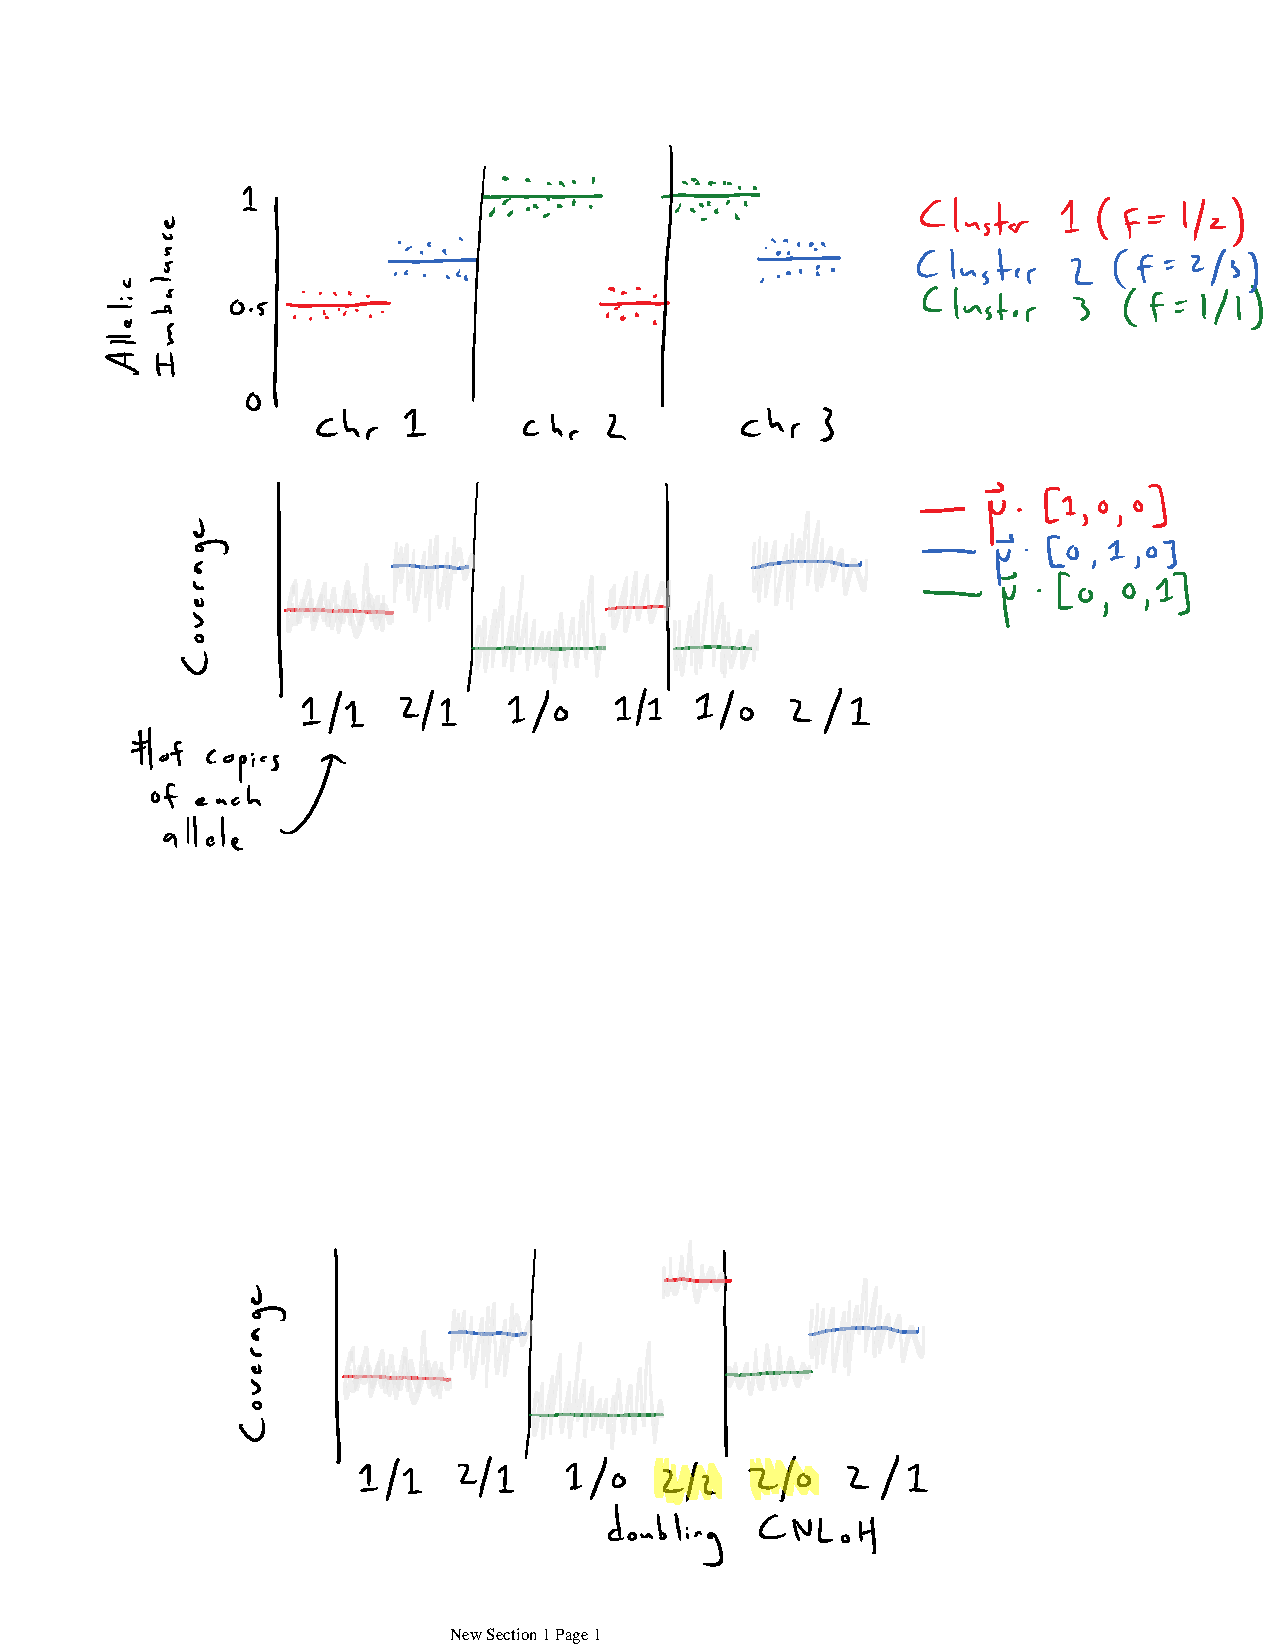
\includegraphics[trim={1cm 13cm 0 3cm},clip,width=10cm]{Figs/fig2.pdf}
\caption{Using allelic imbalance to determine regions that should have the same average coverage, in the absence of balanced events. (Assumes unambiguous assignment of SNPs to clusters, so each $\vec\pi_i$ is one-hot.)}
\label{NormFig}
\end{figure}

In the top panel of Figure \ref{NormFig}, we show a sample with three levels of allelic imbalance at $f=1/2$, $2/3$, and $1$. If there are no balanced gains/losses, these respectively correspond to allelic copy numbers of $1/1$ (i.e., diploid), $2/1$ (i.e., gain of one allele), and $1/0$ (i.e., loss of one allele). We can thus estimate the total copy ratio of each cluster via the total genomic coverage within each cluster. We improve this estimate by regressing out known technical factors that bias coverage.

We achieve this via Poisson regression. Assuming genomic coverage is (overdispersed) Poisson distributed across intervals, then the number of reads in the $i$th interval $r_i$ can be modeled as
\begin{align*}
r_i \sim \textop{Pois}(\exp(\vec\mu\cdot\vec \pi_i + \vec\beta\cdot\vec c_i + \epsilon_i))\qquad \epsilon_i\sim p(\theta),\btag{poiss0}
\end{align*}
where $\vec\pi_i$ is the average cluster assignment probability across all SNPs $S_{i,1},\dots,S_{i,M}$ within interval $i$, i.e.
\begin{align*}
\vec \pi_i=\frac{1}{M}\lt[\sum_{m=1}^M\textop{Pr}[S_{i,m}\in C_1],\dots,\sum_{m=1}^M\textop{Pr}[S_{i,m}\in C_N]\rt],
\end{align*}
with each assignment probability inferred from the clustering procedure described in the previous section. $\vec\mu$ is a free parameter, whose $j$th element corresponds to the mean coverage of each interval within cluster $C_j$. $\vec\beta$ corresponds to the multiplicative effects covariates $\vec c_i$ have on coverage. $\epsilon_i$ is an optional latent random variable representing overdispersion, parameterized by $\theta$.

The likelihood of this model is
\begin{align*}
\mathcal{L}(\vec \mu,\vec\beta,\theta|\{r_i\},\{\vec \pi_i\},\{\vec c_i\}) = \prod_i \int_{\varepsilon} d\epsilon_i \textop{Pois}(r_i;\exp(\vec\mu\cdot\vec \pi_i + \vec\beta\cdot\vec c_i + \epsilon_i))p(\epsilon_i|\theta).
\end{align*}
If we assume no overdispersion, $p(\epsilon|\theta)=1$ and this is an ordinary Poisson regression; the maximum likelihood estimate for the parameters can be easily found via Newton-Raphson optimization. If we add overdispersion, then we should either pick $p(\epsilon_i|\theta)$ such that the integral has closed form (e.g., make it a gamma distribution) or such that a good numerical approximation of the integral has a closed form (e.g., make it a log-normal distribution).

After fitting this model, $\vec\mu\cdot\vec\pi_i$ yields the normalized log coverage for the $i$th interval, after regressing out technical covariates. We show this in the bottom panel of Figure \ref{NormFig}. Note that for simplicity, we assume that each SNP is unambiguously assigned to a cluster, so each $\vec\pi_i$ has one element with probability 1 and every other element with probability 0 (i.e., it is one hot). In reality, while most SNPs will have nearly unambiguous cluster assignments, they are probabilistically assigned, so each interval's expected coverage is also actually probabilistic.

\subsection{Accounting for balanced events}

\begin{figure}
\centering
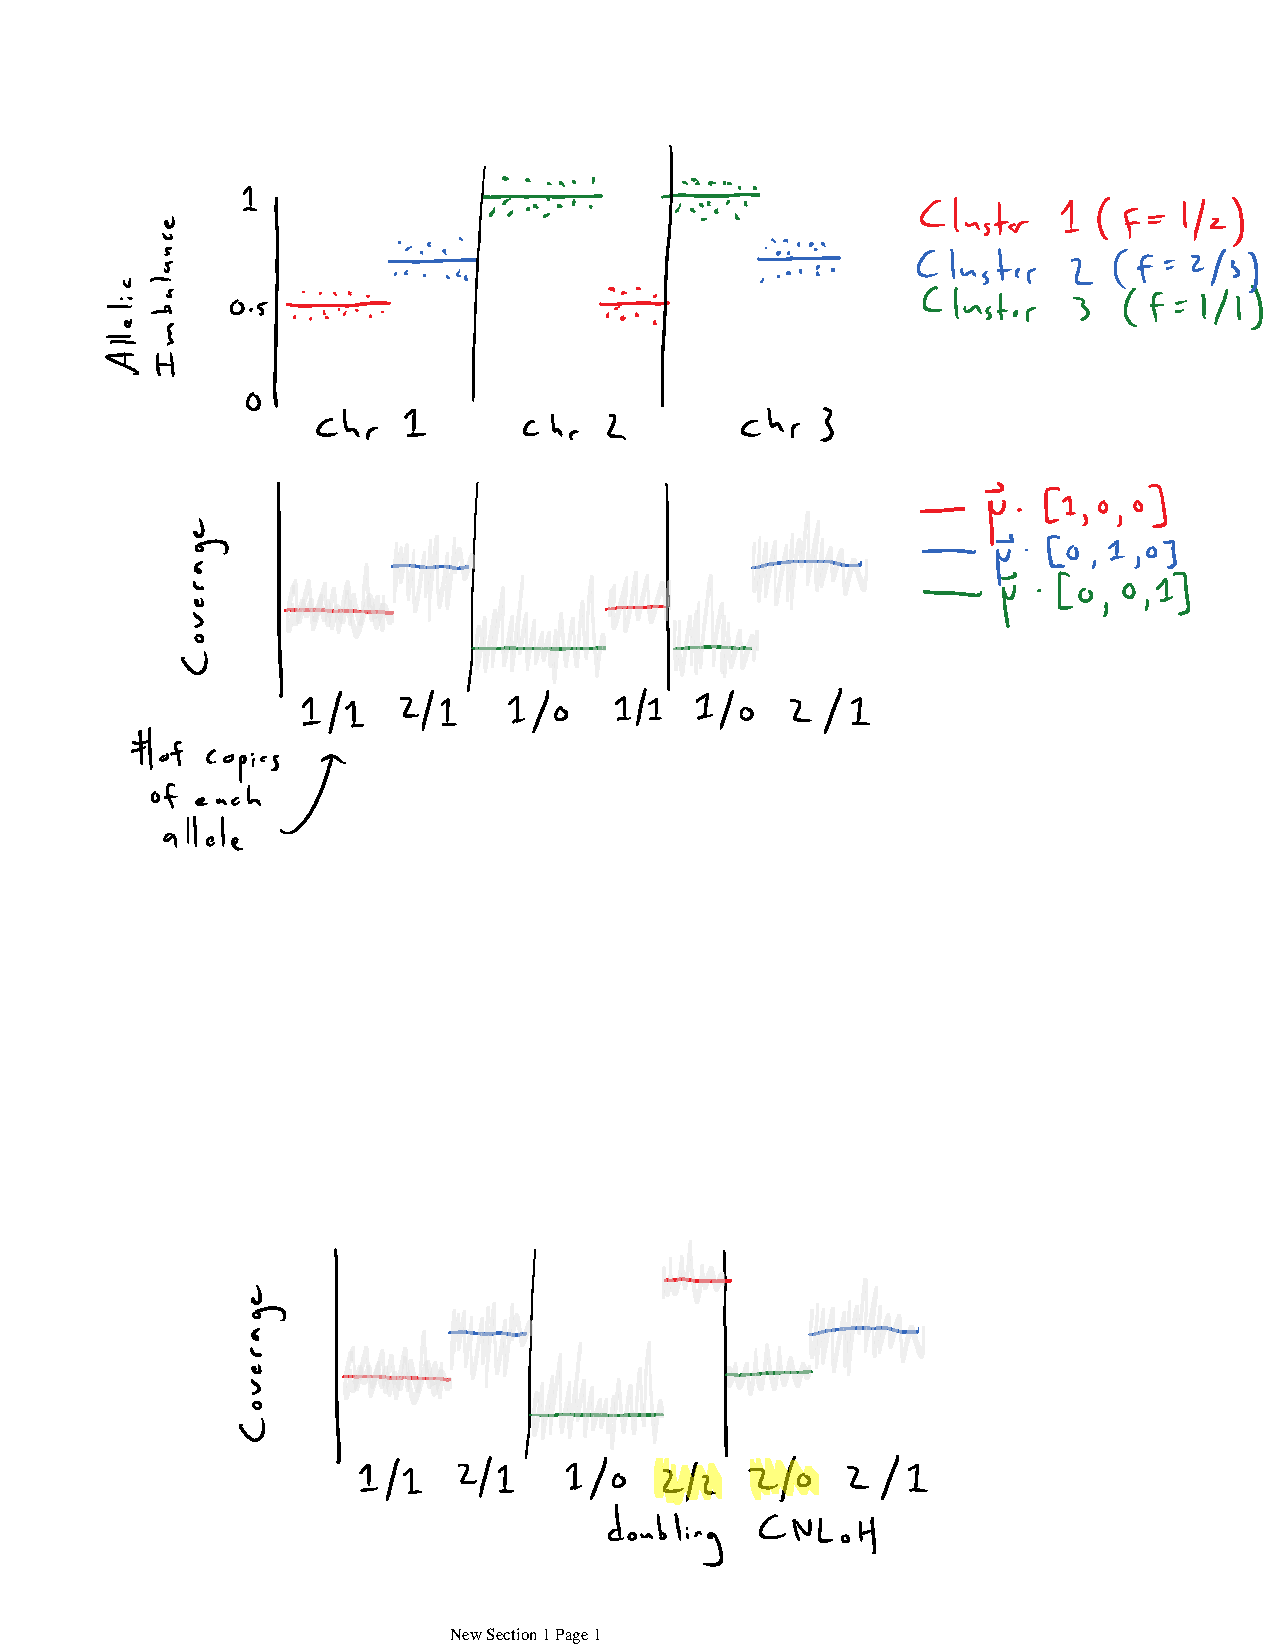
\includegraphics[trim={1.5cm 20cm 6.5cm 3cm},clip,width=10cm]{Figs/fig2.pdf}
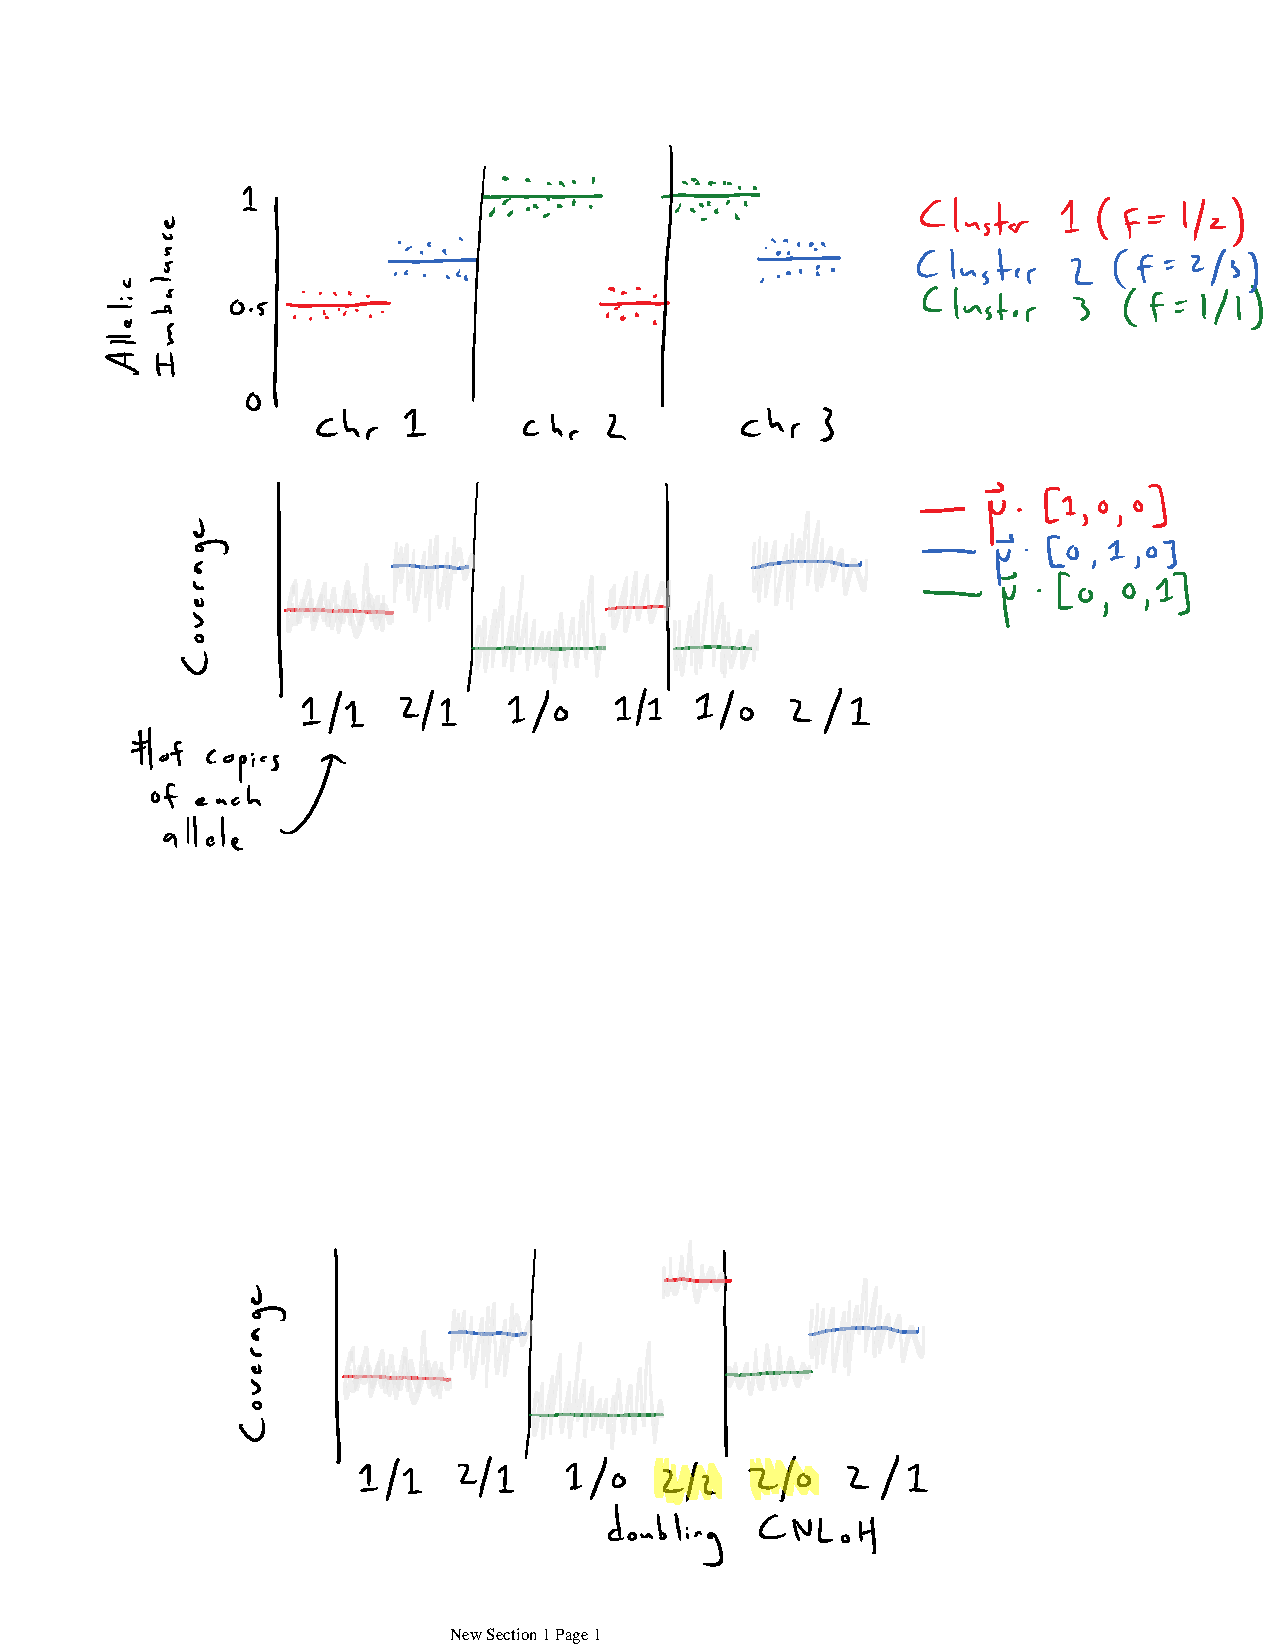
\includegraphics[trim={2.5cm 1cm 5cm 21cm},clip,width=10cm]{Figs/fig2.pdf}
\caption{In the case of balanced events (highlighted in yellow), we cannot assume that the mean coverage for the allelic imbalance cluster the balanced event belongs to will accurately represent its coverage.}
\label{BalancedNormFig}
\end{figure}

The aforementioned model only works in the absence of balanced copy number events (i.e., doubling/CNLoH). For example, if a genomic region gains one copy of each haplotype, it will have the same allelic imbalance as a region without the gain but up to double the genomic mass (if the doubling is clonal). Likewise, a region with CNLoH will have the same allelic imbalance as a region with only one allele.

We therefore cannot assume that there is a one-to-one correspondence between levels of allelic imbalance and levels of total copy ratio (Figure \ref{BalancedNormFig}). To account for this, we need to perform an additional round of segmentation on the normalized coverage.

The proposed procedure for this is as follows. Initially, assume that each interval belongs to its own segment by adding an additional $\mu_i$ term to \eqref{poiss0},
\begin{align*}
r_i \sim \textop{Pois}(\exp(\vec\mu\cdot\vec \pi_i + \mu_i + \vec\beta\cdot\vec c_i + \epsilon_i)).
\end{align*}

The likelihood of our model is thus
\begin{align*}
\mathcal{L}(\vec \mu,\vec\beta,\{\mu_i\},\theta|\{r_i\},\{\vec \pi_i\},\{\vec c_i\}) = \prod_i \underbrace{\int_{\varepsilon} d\epsilon_i \textop{Pois}(r_i;\exp(\vec\mu\cdot\vec \pi_i + \mu_i + \vec\beta\cdot\vec c_i + \epsilon_i))p(\epsilon_i|\theta)}_{p(r_i|\vec\mu,\mu_i,\vec \beta,\vec \pi_i, \vec c_i)}.
\end{align*}

To perform inference on this model, we first fit the simplified model of the previous section, i.e., initialize all $\mu_i$ terms to 0, and optimize $\vec\mu$, $\vec\beta$, and optionally $\theta$, if we are adding overdispersion. We then pick two adjacent intervals $r_j$, $r_{j+1}$ at random, and optimize the likelihood if they are joined,
\begin{align*}
\mathcal{L}(\vec \mu,\vec\beta,\mu_{j,j+1},\theta|\{r_i\},\{\vec \pi_i\},\{\vec c_i\}) &= p(r_j|\vec\mu, \mu_{j,j+1},\vec\beta,\vec \pi_j, \vec c_j)\times p(r_{j+1}|\vec\mu, \mu_{j,j+1},\vec\beta,\vec \pi_{j+1}, \vec c_{j+1})\\
&\phantom{{}=}\times\prod_{i\notin\{j,j+1\}} p(r_i|\vec\mu, \mu_i,\vec\beta,\vec \pi_i, \vec c_i).\btag{seg_join}
%\mathcal{L}(\vec \mu,\vec\beta,\mu_{j,j+1},\theta|\{r_i\}) &= \phantom{{}\times{}}\int_{\varepsilon} d\epsilon_j \textop{Pois}(r_j;\exp(\vec\mu\cdot\vec p_j + \mu_{j,j+1} + \vec\beta\cdot\vec c_j + \epsilon_j))p(\epsilon_j|\theta)\\
%&\phantom{{}={}}\times\int_{\varepsilon} d\epsilon_{j+1}\textop{Pois}(r_{j+1};\exp(\vec\mu\cdot\vec p_{j+1} + \mu_{j,j+1} + \vec\beta\cdot\vec c_{j+1} + \epsilon_{j+1}))p(\epsilon_{j+1}|\theta)\\
%&\phantom{{}={}}\times\prod_{i\notin\{j,j+1\}} \int_{\varepsilon} d\epsilon_i \textop{Pois}(\exp(\vec\mu\cdot\vec p_i + \vec\beta\cdot\vec c_i + \epsilon_i))p(\epsilon_i|\theta).
\end{align*}
Note that $\mu_{j,j+1}$ is shared between the first two terms. Conversely, the likelihood that they are split is
\begin{align*}
\mathcal{L}(\vec \mu,\vec\beta,\mu_{j},\mu_{j+1},\theta|\{r_i\},\{\vec \pi_i\},\{\vec c_i\}) &= p(r_j|\vec\mu, \mu_{j},\vec\beta,\vec \pi_j, \vec c_j)\times p(r_{j+1}|\vec\mu, \mu_{j+1},\vec\beta,\vec \pi_{j+1}, \vec c_{j+1})\\
&\phantom{{}=}\times\prod_{i\notin\{j,j+1\}} p(r_i|\vec\mu, \mu_i,\vec\beta,\vec \pi_i, \vec c_i).\btag{seg_split}
\end{align*}
Here, note that $\mu_j$ and $\mu_{j+1}$ are distinct parameters in the first two terms.

We then compute the marginal likelihoods of \eqref{seg_split} and \eqref{seg_join},
\begin{align*}
\mathcal{M}(\text{join}) &= \int d\vec\mu\,d\vec\beta\,d\mu_{j,j+1}\,d\theta\, \mathcal{L}(\vec \mu,\vec\beta,\mu_{j},\mu_{j+1},\theta|\{r_i\},\{\vec \pi_i\},\{\vec c_i\})\\
\mathcal{M}(\text{split}) &= \int d\vec\mu\,d\vec\beta\,d\mu_{j}\,d\mu_{j+1}\,d\theta\, \mathcal{L}(\vec \mu,\vec\beta,\mu_{j},\mu_{j+1},\theta|\{r_i\},\{\vec \pi_i\},\{\vec c_i\})
\end{align*}
and probabilistically join the adjacent intervals with probability
\begin{align*}
p(\text{join}) = \frac{\mathcal{M}(\text{join})}{\mathcal{M}(\text{join})+\mathcal{M}(\text{split})}.
\end{align*}

%$p(S_{i,j}

%Now suppose that there are many disjoint segments $\mathcal{S}_j\in\{\mathcal{S}\}$, each with a potentially different allelic imbalance. 
%The total likelihood of a given segmentation is
%\begin{align*}
%\mathcal{L}(\{f\}|\{\mathcal{S}\})=\prod_j \mathcal{L}(f_j|\mathcal{S}_j).
%\end{align*}
%
%We want to find the optimal partition of SNPs (i.e., the optimal set $\{\mathcal{S}\}$)
%
%
%The probability that two allelic segments have the same allelic imbalance is the probability that their beta distribution likelihoods
%\begin{align*}
%f_1\sim \textop{beta}(1 + A_1, 1 + B_1) \qquad f_2\sim \textop{beta}(1 + A_2, 1 + B_2) 
%\end{align*}
%are consistent according to the following two-sided test:
%\begin{align*}
%\textop{Pr}(f_1 \sim f_2) = 2\times\min\lt\{\textop{Pr}(f_1 > f_2),\textop{Pr}(f_1 < f_2)\rt\}.
%\end{align*}
%We could obtain this via convolution, since for $X\sim p$ and $Y\sim q$, we have
%\begin{align*}
%\textop{Pr}(X > Y) = \textop{Pr}(X - Y > 0) = \int_0^\infty d\phi\,\int_{\mathbf{\Theta}} d\theta\,p(\theta)q(\theta - \phi),
%\end{align*}
%but in practice it is cheap enough to obtain via Monte Carlo simulation of the two beta random variables. We draw $n$ samples from $f_1$ and $f_2$ and empirically compute the fraction $\sum_{i=1}^n\bs{1}(f^{(1)}_i > f^{(2)}_i)/n$ for $f_{1\dots n}^{(1)}\sim f_1$ and $f_{1\dots n}^{(2)}\sim f_2$, where $\bs 1$ is the indicator function.
%
%We can sample the posterior probability of segment boundaries via a Metropolis-like sampler. The marginal likelihood of a given set of segments $S$ is
%\begin{align*}
%\mathcal{M}(s) &= \prod_{i\in S} \int_0^1 df\,f^{1 + A_i}(1 - f)^{1 + B_i}\\
%&= \prod_i \beta(A_i, B_i).
%\end{align*}
%We probabilistically propose a new segmentation $S^\ast$ from distribution $q(S^\ast|S)$, and accept $S^\ast$ with probability
%\begin{align*}
%\textop{Pr}(S\to S^\ast) = \min\lt\{1,\frac{\mathcal{M}(S^\ast)q(S|S^\ast)}{\mathcal{M}(S)q(S^\ast|S)}\rt\}
%\end{align*}
%todo: what if $q$ is asymmetric?
%
%For simplicity, let's first assume we have perfect phasing accuracy across an entire chromosome. We initialize each SNP belonging to its own segment. At random, we select two adjacent segments and merge them with probability $p_\text{merge}=\textop{Pr}(f_1 \sim f_2)$, or keep them separate with probability $1 - p_\text{merge}$. If we merge two segments, we compute the marginal likelihood 
%
%\section{Misphasing}
%
%Because we generally do not know perfect phasing information (which would require haplotype-resolved sequencing, e.g., with a parental trio or long reads), we must impute it from a reference panel. Assignment to haplotype $\mathcal{A}$ and $\mathcal{B}$ are therefore not consistent along the entire length of a chromosome arm, but only within small regions (known as ``phase sets'') much smaller than a typical LD block. The SNPs within a given phase set are relative to the haplotypes $\mathcal{A}_i$ and $\mathcal{B}_i$ within that set; we do not know whether $\mathcal{A}_i$ and $\mathcal{A}_j$ belonging to different phase sets are on the same physical molecule.
%
%Furthermore, there is the chance that an individual SNP within a phase set is misphased.
%
%Around a potential phase set boundary, we have four haplotypes $\mathcal{A}_1$, $\mathcal{B}_1$, $\mathcal{A}_2$, and $\mathcal{B	}_2$, with total respective read counts $A_1$, $B_1$, $A_2$, and $B_2$. Suppose the boundary represents a true 
%
%Let $m$ be a binary indicator variable that the break represents a true misphasing. Then by Bayes' rule, the probability of a misphase given the observed readcounts is
%
%\begin{align*}
%p(m|A_1, A_2, B_1, B_2) = \frac{p(A_1, A_2, B_1, B_2|m)p(m)}{\sum_m p(A_1, A_2, B_1, B_2|m)p(m)}
%\end{align*}
%
%Transitions:
%\begin{align*}
%p(f_1 \sim f_2, m|A_1,B_1,A_2,B_2) = p(f_1 \sim f_2|m,A_1,B_1,A_2,B_2)p(m|A_1,B_1,A_2,B_2)
%\end{align*}
%
%\begin{align*}
%f_1 \sim f_2, m=0\\
%f_1 \nsim f_2, m=0\\
%f_1 \sim f_2, m=1\\
%f_1 \nsim f_2, m=1
%\end{align*}
%
%\section{Splitting}
%
%For a given segment comprising $n$ SNPs with total readcounts $A_\mathcal{S}$ on haplotype $\mathcal A$ and $B_\mathcal{S}$ on haplotype $\mathcal B$, the likelihood of breaking it at position $b \in \{1\dots n\}$ is
%\begin{align*}
%\mathcal{L}(b|A_\mathcal{S},B_\mathcal{S}) &= \int_0^1 df\,f^{1 + A_{1\dots b}}(1 - f)^{1 + B_{1\dots b}}\times \int_0^1 df\,f^{1 + A_{b + 1\dots n}}(1 - f)^{1 + B_{b + 1\dots n}}\\
%&= \beta(A_{1\dots b}, B_{1\dots b})\beta(A_{b + 1\dots n},B_{b + 1\dots n})
%\end{align*}
%where $A_{i\dots j}$ is the sum of readcounts from SNP $i$ to $j$ on haplotype $\mathcal A$. The probability of choosing a given $b$ is thus
%\begin{align*}
%p(b|A_\mathcal{S},B_\mathcal{S}) = \frac{\mathcal{L}(b|A_\mathcal{S},B_\mathcal{S})}{\sum_{i=1}^n \mathcal{L}(i|A_\mathcal{S},B_\mathcal{S})}.
%\end{align*}

\end{document}